%% This is an example first chapter.  You should put chapter/appendix that you
%% write into a separate file, and add a line \include{yourfilename} to
%% main.tex, where `yourfilename.tex' is the name of the chapter/appendix file.
%% You can process specific files by typing their names in at the 
%% \files=
%% prompt when you run the file main.tex through LaTeX.
\chapter{Infrastructure}

This chapter aims to describe the tools and processes involved in the infrastructure setup, from local development environment to the set of production servers running the Redch. Firstly, it explains the infrastructure setup and secondly, describes the provisioning and deployment processes.

\section{Amazon AWS setup}

Amazon Web Services (AWS) is a cloud computing platform. It offers a collection of remote computing services ranging from computing and storage to networking services such as DNS, among others. AWS is a world-wide leader of Infrastructure-as-a-Service (IaaS) providers with numerous companies like Spotify, Heroku, Airbnb, Foursquare, Github, Reddit or Mapbox relying on them.

The whole infrastructure of the system is made up of EC2 instances, virtual servers in Amazon's cloud. They all run a custom Amazon Machine Image (AMI) built from a raw Ubuntu 12.04 LTS with all needed dependencies ---Puppet and Ruby 2.0.0--- installed. As a result, any new instance booted up with this custom AMI is ready to be provisioned. Starting and stopping machines, as well as configuring their firewall rules is managed through the AWS Management Console, a web UI.

One of the major benefits Redch can take advantage of is Amazon's Auto Scaling. This service allows to scale the capacity of the EC2 instances up and down according to a set of predefined conditions. A load balancer, for instance, can automatically spawn app servers during demand spikes and shut them down during low demand periods. Redch can get the most out of it by exploiting the fact that solar panels don't produce energy at night, thereby minimizing costs. Likewise, less computing power is required under windless conditions.

Although it would desirable to keep a provider-independent infrastructure, Amazon RDS has been chosen as database server which makes it easier to set up, operate and scale a relational database. Furthermore, it provides automated backups, Multi-AZ replication and monitoring metrics. It has support for MySQL, Oracle, SQL Server and PostrgeSQL, all the DBMSs supported by 52ºNorth SOS, being the latter the one it uses by default. However, the PostrgeSQL support is still in beta version due to its recent release in November of 2013.

The final production environment consists of the four servers shown in \ref{fig:infrastructure}. Three EC2 micro instances plus a RDS micro instance. Amazon's free tier includes both services at no cost within the first year. Therefore, EC2 micro instances are limited to 1 low-capacity throttled CPU with 627MB of RAM \footnote{AWS Micro Instances Documentation: \url{http://docs.aws.amazon.com/AWSEC2/latest/UserGuide/concepts_micro_instances.html}}. All three EC2 instances are attached to an 8GB Elastic Block Storage (EBS), which are storage volumes with built-in redundancy. These volumes host the filesystem of their related EC2 instances.

\begin{sidewaysfigure}
  \centering
  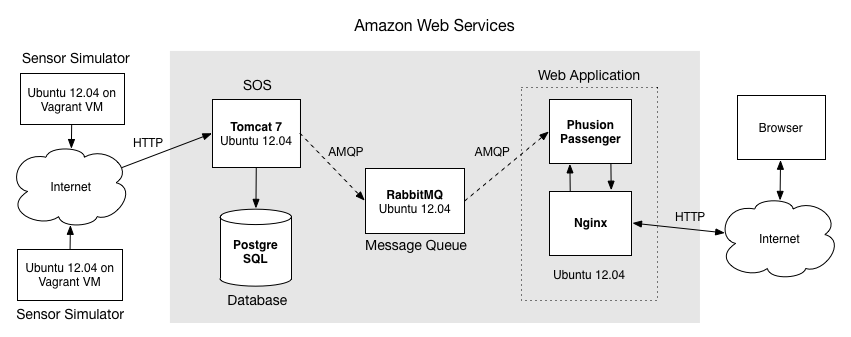
\includegraphics[width=\textwidth]{infrastructure}
  \caption{Production's infrastructure diagram}
  \label{fig:infrastructure}
\end{sidewaysfigure}

Ubuntu 12-04 LTS has been chosen as the OS of all three servers due to its stability and security as well as the inherent benefits of a Linux OS. With regard to the database, Amazon's RDS abstract away from the particularities of the underlying hardware by providing the database access as a service.

\section{Provisioning}

Once the software is developed, the underlying infrastructure must be configured to host each of the system components. This process, which involves creating directories and installing packages, may be error-prone when done manually. Besides, the process may need to be repeated several times whenever new servers are set up. Although writing down the build-out process may help, whoever reads that documentation may not be able to figure out the current state of the configuration.

Server automation frameworks formalize systems administration treating infrastructure as code. As a result, infrastructure configuration can be tested and repeated, automating away repetitive tasks while systems administrators focus on architecting and tunning services.

Puppet, among other solutions such as Chef, enables server configuration automation. It automates server provisioning by formalizing its configuration into manifests. Puppet's manifests are text files that contain statements written in a declarative DSL that allows the desired state of the infrastructure to be defined. Once these configurations are deployed, Puppet automatically installs the necessary packages and ensures that the machine’s files and services match the desired state.

\begin{listing}[h]
\begin{minted}[
frame=lines,
framesep=2mm,
baselinestretch=1.2,
fontsize=\footnotesize,
linenos
] {puppet}
package { 'apache2':
  provider => 'apt',
  ensure   => 'installed'
}

service { 'apache2':
  ensure => 'running'
}
\end{minted}
\caption{Example of Puppet's manifest file}
\label{fig:puppet}
\end{listing}

Puppet is mature and widely used. Besides having an open source version, there are lots of learning materials available online.

Prior provisioning, any server must have Puppet installed. This comes packaged as a ruby gem and therefore, also requires a MRI Ruby interpreter. Puppet can be installed with any system package manager, doing so will likely install previous releases missing features and bug fixes.

Puppet enables provision machines by either applying the configuration directly or compiling into a catalog and distributing it to the target system via a client-server paradigm.

\subsection*{Production Software}

Most of the software used in the development environment is also used in the production. This is the case of SOS, for instance, where both Tomcat 7 and PostgreSQL have been chosen to run also in production. However, the production web application stack differs from the one used in development. Nginx plus Passenger has been chosen over Thin, the server included in Sinatra for development purposes.

Passenger is a mature and feature-rich application server widely used in many production scenarios. Therefore, is easy to find learning materials and support on the internet. Nginx on the other hand, is a high-performance web server and load balancer that can handle high concurrency.

Placed in front of the application server, Nginx acts as a reverse-proxy. It deals with all incoming requests serving static files efficiently and passing them to the application layer. Passenger then processes the requests and returns a response.

\section{Deployment}

Once the configuration is applied, the target server is up and ready. Next, the code release must be transferred to the production environment to make the application available for use.

Capistrano is a remote multi-server automation tool that enables the execution of arbitrary tasks on remote servers over SSH. It aims to allow reliable deployment of web applications to any number of machines simultaneously. All of its features enforce sane development workflows.

The general configuration of the application is set in the \texttt{deploy.rb} file. Then, each particular stage overrides it in its own file. By following this convention, Capistrano infers the environment names and enables tasks to be run on each of them as in \ref{fig:capistrano}.

\begin{listing}[h]
\begin{minted}[
frame=lines,
framesep=2mm,
baselinestretch=1.2,
fontsize=\footnotesize,
linenos
] {ruby}
set :application, 'redch'
set :repo_url, 'git://github.com/sauloperez/redch-webapp.git'
set :ssh_options, {
  forward_agent: true
}

ask :branch, proc { `git rev-parse --abbrev-ref HEAD`.chomp }

set :deploy_to, '/var/redch'
set :use_sudo, false
set :deploy_via, :copy
set :copy_strategy, :export

SSHKit.config.command_map[:rake]  = "bundle exec rake"

after 'deploy:publishing', 'nginx:restart'
after 'deploy:publishing', 'passenger:restart'
\end{minted}
\caption{Capistrano's deployment definition}
\label{fig:deploy.rb}
\end{listing}

\begin{figure}[h]
  \texttt{\$ cap staging deploy}\\
  \texttt{...}\\
  \texttt{\$ cap production deploy:rollback}\\
  \caption{Execution of commands in different environments}
  \label{fig:capistrano}
\end{figure}

The configuration can be tailored to fit the needs of the project by writing extra tasks. Capistrano provides the \textit{deploy} and \textit{rollback} flows that invoke several hooks for the developer to hook up custom tasks into the flow either before or after the particular hook. In line 16 of listing \ref{fig:deploy.rb} Nginx is restarted right after the release has been published and before the deploy's leftovers are cleaned up.

Therefore, some custom Capistrano tasks have been developed to ease the execution of common operations such as starting and stopping tomcat. The listing \ref{fig:cap_nginx} illustrates Nginx-related tasks used in the web application's deployment.

\begin{listing}[h]
\begin{minted}[
frame=lines,
framesep=2mm,
baselinestretch=1.2,
fontsize=\footnotesize,
linenos
] {ruby}
namespace :nginx do
  desc 'Start nginx'
  task :start do
    on roles(:app), in: :sequence, wait: 5 do
      sudo 'start nginx'
    end
  end

  desc 'Stop nginx'
  task :stop do
    on roles(:app), in: :sequence, wait: 5 do
      sudo 'stop nginx'
    end
  end

  desc 'Restart nginx'
  task :restart do
    on roles(:app), in: :sequence, wait: 5 do
      sudo 'restart nginx'
    end
  end
end
\end{minted}
\caption{Content of \texttt{lib/capistrano/tasks/nginx.cap}}
\label{fig:cap_nginx}
\end{listing}

As Capistrano essentially executes commands in a remote server, custom tasks can written to target any specific purposes such as listing servers' uptimes, checking their load, etc.